\documentclass[letter,11pt]{article}

\usepackage[spanish,es-nodecimaldot]{babel}
\usepackage[utf8]{inputenc}

\usepackage{lmodern}
\usepackage[T1]{fontenc}
\usepackage{textcomp}

\usepackage{framed}
\usepackage[svgnames]{xcolor}
\colorlet{shadecolor}{Gainsboro!50}

\usepackage[labelfont=bf]{caption}
\usepackage{graphicx}
\usepackage{pstricks}

\usepackage{anysize}
\marginsize{3cm}{2cm}{2cm}{3cm}

\usepackage{siunitx}
\usepackage{amsmath}
\usepackage{array}
\usepackage{alltt}
\usepackage{xcolor,colortbl}

\definecolor{silver}{rgb}{0.752,0.752,0.752}
\definecolor{gold}{rgb}{0.811,0.709,0.231}

\usepackage{fancyhdr}
\usepackage{lastpage}
\pagestyle{fancy}
\fancyhf{}
\fancyhead[LE,RO]{Laboratorio de Física Básica III}
\fancyfoot[CO,CE]{\thepage\ de \pageref{LastPage}}

\special{papersize=215.9mm,279.4mm}

\usepackage[
    pdfauthor={
        Bastos Lizondo Rosemary;
        Blanco Alconz John Brandon;
        Caballero Burgoa Carlos Eduardo;
        Villena Gutiérrez Ismael Cristian
    },%
    pdftitle={Laboratorio de Física Básica III},%
    pdfsubject={Mediciones de la resistencia eléctrica},%
    colorlinks,%
    citecolor=black,%
    filecolor=black,%
    linkcolor=black,%
    urlcolor=black,
    breaklinks]{hyperref}
\usepackage{breakurl}

\newcommand{\blankpage}{
\newpage
\thispagestyle{empty}
\mbox{}
\newpage
}

\renewcommand{\arraystretch}{1.2}

\begin{document}

\begin{titlepage}
\begin{center}
{\Large UNIVERSIDAD MAYOR DE SAN SIMÓN}\\
\vspace*{0.15cm}
{\large FACULTAD DE CIENCIAS Y TECNOLOGÍA}\\
\vspace*{0.10cm}
DEPARTAMENTO DE FÍSICA\\
\vspace*{3.0cm}
{\Large \textbf{LABORATORIO DE FÍSICA BÁSICA III}}\\
\vspace*{0.3cm}
{\Large \textbf{INFORME No. 4}}\\
\vspace*{3.5cm}
{\Large \textbf{MEDICIONES DE LA RESISTENCIA ELÉCTRICA}}\\
\end{center}

\vspace*{5.8cm}
\leftskip=7.95cm
\noindent
\textbf{Integrantes:}\\
Bastos Lizondo Rosemary.\\
Blanco Alconz John Brandon.\\
Caballero Burgoa Carlos Eduardo.\\
Villena Gutiérrez Ismael Cristian.\\
\newline
\textbf{Docente:}\\
Ing. Flores Flores, Freddy.\\
\newline
\textbf{Grupo:} G3.\\
\textbf{Fecha de entrega:} 15 de Abril del 2021.\\

\end{titlepage}

\section{Preguntas previas}
\begin{enumerate}
\item \textbf{¿Qué función tiene una resistencia eléctrica en un circuito
eléctrico?} \\
La resistencia eléctrica es la completa oposición que encuentra la corriente a
su paso por un circuito eléctrico cerrado, atenuando o frenando el libre flujo
de circulación de las cargas eléctricas o electrones. Cualquier dispositivo o
consumidor conectado a un circuito eléctrico representa en sí una carga,
resistencia u obstáculo para la circulación de la corriente eléctrica.

\item \textbf{¿Con qué propiedad de la materia está relacionada la resistencia
eléctrica?} \\
Con la resistividad eléctrica, que mide su capacidad para oponerse al flujo de
carga eléctrica a través de ella. Un material con una resistividad eléctrica
alta (conductividad eléctrica baja), es un aislante eléctrico y un material con
una resistividad baja (conductividad alta) es un buen conductor eléctrico.

\item \textbf{¿Qué tipos de resistencias existen?} \\
Hay dos tipos básicos de resistencias:

\begin{itemize}
    \item Resistencias lineales.
        \begin{itemize}
            \item Resistencias fijas.
                \begin{itemize}
                    \item Resistencias de composición de carbono.
                    \item Resistores de alambre enrollado.
                    \item Resistores de película delgada.
                        \begin{itemize}
                            \item Resistencias de película de carbono.
                            \item Resistores de película de metal.
                        \end{itemize}
                    \item Resistores de película gruesa.
                        \begin{itemize}
                            \item Resistencias de óxido de metal.
                            \item Resistores de película \emph{Cermet}.
                            \item Resistencias fusibles.
                        \end{itemize}
                \end{itemize}
            \item Resistencias variables.
                \begin{itemize}
                    \item Potenciómetros.
                    \item Reóstatos.
                    \item Recortadores.
                \end{itemize}
        \end{itemize}
    \item Resistencias no lineales.
        \begin{itemize}
            \item Termistor.
            \item Varistores (VDR).
            \item Resistencia fotográfica o célula fotoconductora o LDR.
        \end{itemize}
\end{itemize}

\item \textbf{¿Qué métodos existen para determinar la resistencia eléctrica de
un resistor?} \\
Pueden clasificarse como:
\begin{itemize}
    \item Medición directa:
    \begin{itemize}
        \item Con un óhmetro.
        \item Basado en el código de colores.
    \end{itemize}
    \item Medición indirecta.
    \begin{itemize}
        \item Voltímetro - amperímetro.
        \item Puente de \emph{Wheatstone}.
    \end{itemize}
\end{itemize}

\end{enumerate}

\section{Objetivos}
\begin{itemize}
\item Determinar por diferentes métodos el valor de la resistencia eléctrica.
\item Determinar la resistencia equivalente de combinaciones de resistencias en
    serie y en paralelo.
\end{itemize}

\section{Fundamento teórico}

La resistencia eléctrica de un material es una medida de la oposición al paso de
la corriente eléctrica, su unidad en el sistema internacional es el ohmio
($\Omega$), y su valor depende de su geometría y de factores externos, como ser
la temperatura. La resistencia eléctrica de un alambre de longitud $L$ y sección
transversal $A$ es:

\begin{equation}
    R = \rho \frac{L}{A}
\label{resistividad}
\end{equation}

Donde $\rho$ es la resistencia eléctrica y su unidad es [$\Omega m$], su valor
depende del tipo de material.

Existen diferentes métodos para la medición de la resistencia eléctrica, algunas
de ellas son:

\begin{itemize}
    \item Voltímetro - Amperímetro (Ley de \emph{Ohm}).
    \item Óhmetro (multímetro).
    \item Código de colores (resistencia de carbón).
    \item Puente de \emph{Wheatstone} (puente de hilo).
\end{itemize}

\subsection{Método I: Voltímetro - amperímetro}
Si se conoce la corriente que circula por un conductor, y la diferencia de
potencial entre sus extremos, entonces a partir de la ley de \emph{Ohm}, se
puede conocer el valor de la resistencia eléctrica del conductor:

\begin{equation}
    R = \frac{V}{I}
\label{ohm}
\end{equation}

\subsection{Método II: Óhmetro}
El óhmetro es un dispositivo electrónico que sirve para medir resistencias
eléctricas. Generalmente, en los multímetros los óhmetros están integrados, y
además de poder medir la resistencia eléctrica, se puede probar continuidad en
los componentes eléctricos.

Para medir la resistencia eléctrica, se debe asegurar que no circule corriente
eléctrica por el circuito, o si es posible aislar el resistor. Luego escoger la
escala adecuada para realizar la medición (se comienza siempre en la escala
mayor).

\subsection{Método III: Código de colores}
Una forma de conocer el valor de una resistencia eléctrica es por medio de
código de colores, por ejemplo, en la \textbf{Figura \ref{figura1}} se observa
un resistor con cuatro franjas. Los diferentes colores tienen un valor numérico,
los cuales están tabulados en la \textbf{Cuadro \ref{cuadro1}}.

\begin{figure}[!h]
\centering
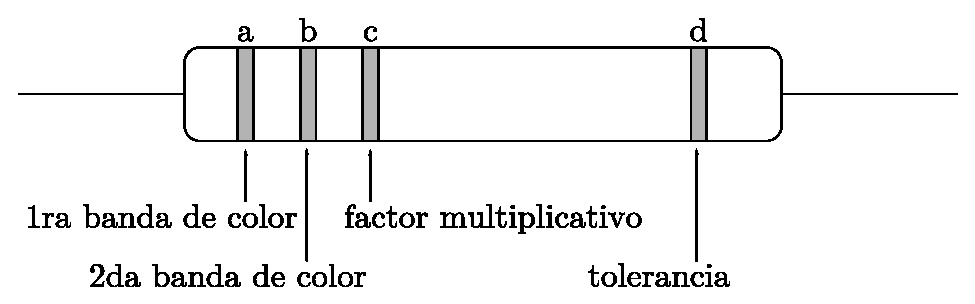
\includegraphics[scale=0.65]{resources/figura1.eps}
\caption{Bandas de color en una resistencia.}
\label{figura1}
\end{figure}

\begin{table}[!h]
\begin{center}
\begin{tabular}{|l|>{\centering}m{1.6cm}<{\centering}
                  |>{\centering}m{2.8cm}<{\centering}
                  |>{\centering}m{2.8cm}<{\centering}
                  |>{\centering}m{2.8cm}<{\centering}|}
\hline
& Color & 1er y 2do dígito & Multiplicador & Tolerancia \tabularnewline \hline
Negro     & \cellcolor{black}  & 0 & $\times 10^0$ & \tabularnewline \hline
Marrón    & \cellcolor{brown}  & 1 & $\times 10^1$ & $\pm 1\%$    \tabularnewline \hline
Rojo      & \cellcolor{red}    & 2 & $\times 10^2$ & $\pm 2\%$    \tabularnewline \hline
Naranja   & \cellcolor{orange} & 3 & $\times 10^3$ &              \tabularnewline \hline
Amarillo  & \cellcolor{yellow} & 4 & $\times 10^4$ &              \tabularnewline \hline
Verde     & \cellcolor{green}  & 5 & $\times 10^5$ & $\pm 0.5\%$  \tabularnewline \hline
Azul      & \cellcolor{blue}   & 6 & $\times 10^6$ & $\pm 0.25\%$ \tabularnewline \hline
Violeta   & \cellcolor{violet} & 7 & $\times 10^7$ & $\pm 0.1\%$  \tabularnewline \hline
Gris      & \cellcolor{gray}   & 8 & $\times 10^8$ & $\pm 0.05\%$ \tabularnewline \hline
Blanco    & \cellcolor{white}  & 9 & $\times 10^9$ &              \tabularnewline \hline
Oro       & \cellcolor{gold}   &   & $\times 0.1$  & $\pm 5\%$    \tabularnewline \hline
Plata     & \cellcolor{silver} &   & $\times 0.01$ & $\pm 10\%$   \tabularnewline \hline
Sin color & \cellcolor{white}  &   &               & $\pm 20\%$   \tabularnewline \hline
\end{tabular}
\caption{Valores nominales, multiplicadores y tolerancias para el código de colores.}
\label{cuadro1}
\end{center}
\end{table}

A partir de la \textbf{Figura \ref{figura1}} el valor de la resistencia
eléctrica es:

\begin{equation}
    R = ab \times c [\Omega]
\label{color}
\end{equation}

y con el valor de la tolerancia se puede encontrar el valor de su error.

\subsection{Método IV: Puente de \emph{Wheatstone}}
El puente de \emph{Wheatstone} es un circuito compuesto por cuatro resistores
(\textbf{Figura \ref{figura2}}), se utiliza para encontrar valores precisos de
la resistencia eléctrica.

\begin{figure}[!h]
\centering
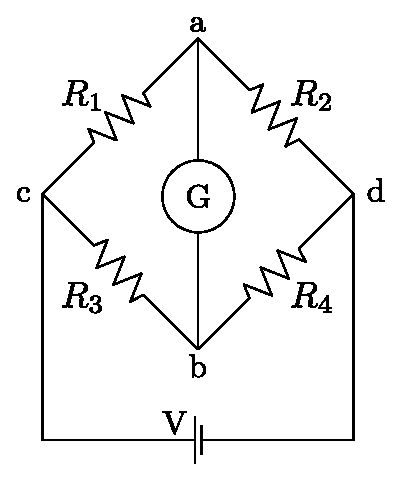
\includegraphics[scale=0.75]{resources/figura2.eps}
\caption{Circuito del puente de \emph{Wheatstone}.}
\label{figura2}
\end{figure}

El puente de \emph{Wheatstone} está en equilibrio cuando la diferencia de
potencial entre $a$ y $b$ es cero y/o cuando la corriente que circula por el
galvanómetro es cero:

\begin{equation}
    I_G = V_{ab} = 0
\label{wheatstone}
\end{equation}

La \textbf{ecuación \ref{wheatstone}} indica que la corriente $I_1$ es igual a
$I_2$, asimismo la corriente $I_3$ es igual a $I_4$. Por tanto en el equilibrio
se tiene:

\begin{equation}
    V_{ca} = V_{cb}; R_1 I_1 = R_3 I_2
\label{vca}
\end{equation}

\begin{equation}
    V_{ad} = V_{bd}; R_2 I_1 = R_4 I_4
\label{vad}
\end{equation}

Si $R_x = R_1$ (resistencia desconocida), y utilizando las ecuaciones
\ref{vca} y \ref{vad} se tiene:

\begin{equation}
    R_x = R_2 \left(\frac{R_3}{R_4}\right)
\label{rx}
\end{equation}

\subsection{Combinación de resistencias eléctricas}

\subsubsection{Combinación en serie}
La resistencia equivalente para una combinación en serie de $n$ resistencias es:

\begin{equation}
    R_{eq} = R_1 + R_2 + R_3 + ... + R_n
\label{serie}
\end{equation}

\subsubsection{Combinación en paralelo}
La resistencia equivalente para una combinación en paralelo de $n$ resistencias
es:

\begin{equation}
    \frac{1}{R_{eq}} = \frac{1}{R_1} + \frac{1}{R_2} + \frac{1}{R_3} + ... + \frac{1}{R_n}
\label{paralelo}
\end{equation}

\section{Materiales}
\begin{itemize}
\item Simulador «PhET Interactive Simulations» Kit de Construcción de Circuitos:
CD - Laboratorio Virtual.
\end{itemize}

\section{Procedimiento experimental}

\subsection{Voltímetro - Amperímetro}

\begin{enumerate}
\item Hacer circular corriente por $R_a$.
\item Medir la corriente eléctrica y el voltaje en la resistencia $R_a$.
\item Con la ley de \emph{Ohm}, determinar el valor de la resistencia $R_a$.
\item Repetir los pasos anteriores para las otras resistencias: $R_b$, $R_c$,
$R_d$, $R_e$.
\end{enumerate}

\subsection{Óhmetro}

La medición directa por medio del Óhmetro, no se llevará a cabo al no contar con
el instrumento en el simulador que se está usando.

\subsection{Código de colores}

A partir de la información del \textbf{Cuadro \ref{cuadro1}} y la
\textbf{Ecuación \ref{color}}, determinar los valores de las resistencias:
$R_a$, $R_b$, $R_c$, $R_d$, $R_e$ con sus respectivos errores.

\subsection{Puente de \emph{Wheatstone}}

\begin{enumerate}
\item Armar el circuito de la \textbf{Figura \ref{figura2}}.
\item Establecer la resistencia cuyo valor desconocemos, entre los puntos
    $a$ y $c$.
\item Colocar tres resistencias cuyo valor sea conocido entre los otros puntos.
\item Intercambiar los valores de estas resistencias conocidas, hasta que la
    diferencia de potencial entre los puntos $a$ y $b$, sea 0 [V].
\end{enumerate}

\subsection{Combinación de resistencias en serie}

\begin{enumerate}
\item Armar las resistencias una tras otra como en la
    \textbf{Figura \ref{figura3}}.
\item Medir el valor de la diferencia de potencial con un voltímetro.
\item Medir la intensidad de corriente con un amperímetro.
\item Calcular la resistencia equivalente de la serie de resistencias con la
    ley de \emph{Ohm}.
\item Calcular la resistencia teórica con la \textbf{Ecuación \ref{serie}}.
\end{enumerate}

\begin{figure}[!h]
\centering
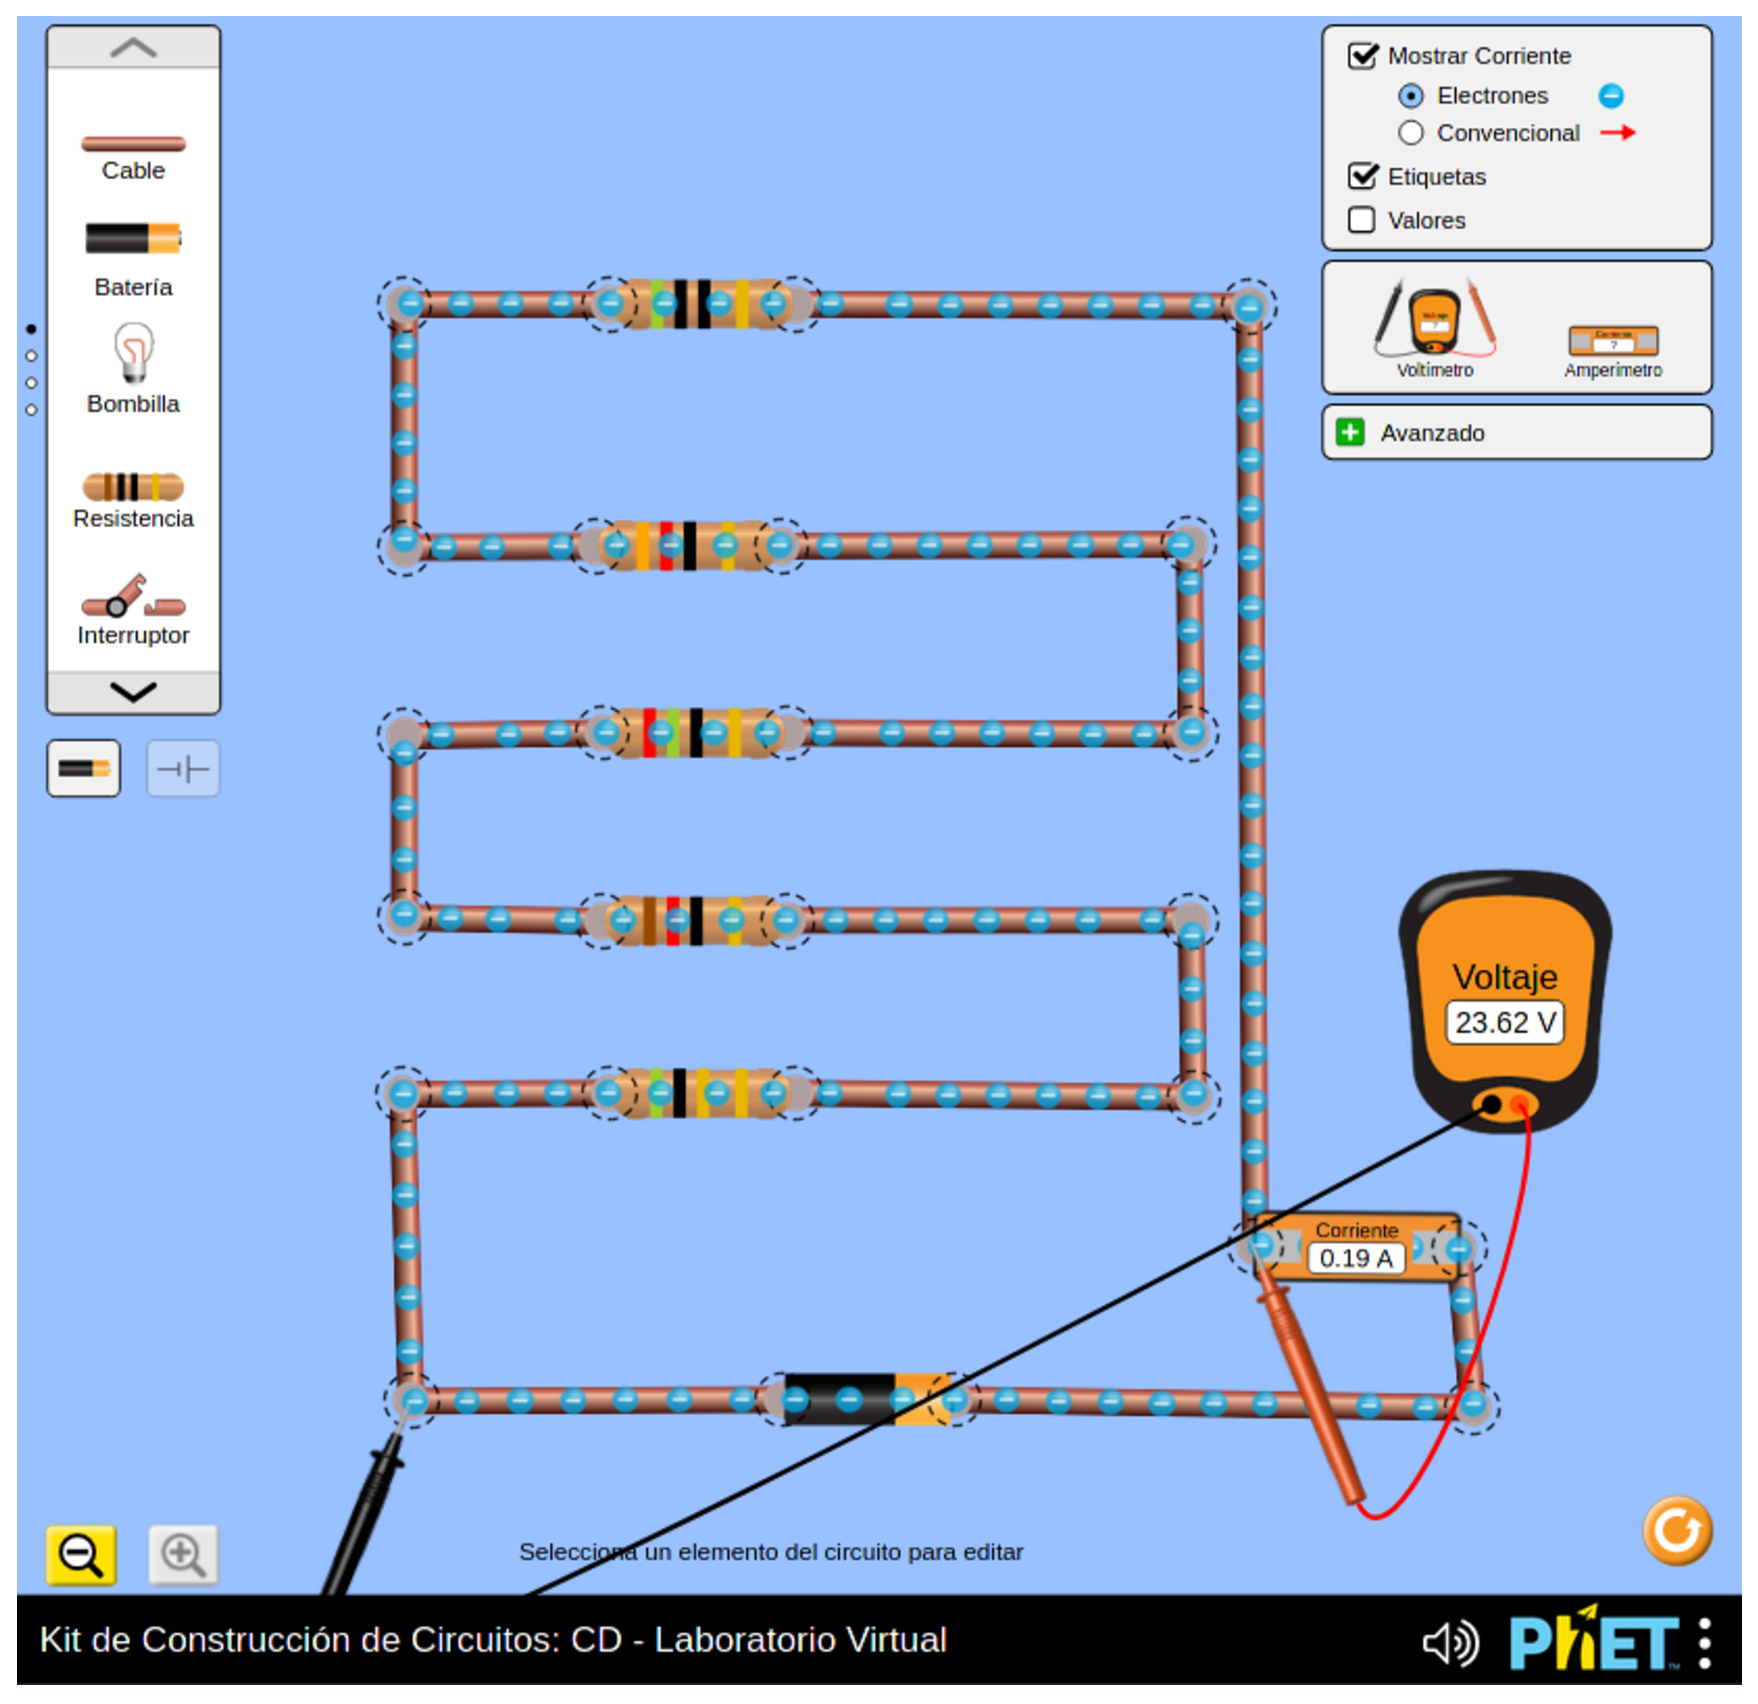
\includegraphics[scale=0.45]{resources/figura3.eps}
\caption{Armado de resistencias en serie.}
\label{figura3}
\end{figure}

\subsection{Combinación de resistencias en paralelo}

\begin{enumerate}
\item Armar las resistencias en paralelo como en la
    \textbf{Figura \ref{figura4}}.
\item Medir el valor de la diferencia de potencial con un voltímetro.
\item Medir la intensidad de corriente con un amperímetro.
\item Calcular la resistencia equivalente de las resistencias en paralelo con
    la ley de \emph{Ohm}.
\item Calcular la resistencia teórica con la \textbf{Ecuación \ref{paralelo}}.
\end{enumerate}

\begin{figure}[!h]
\centering
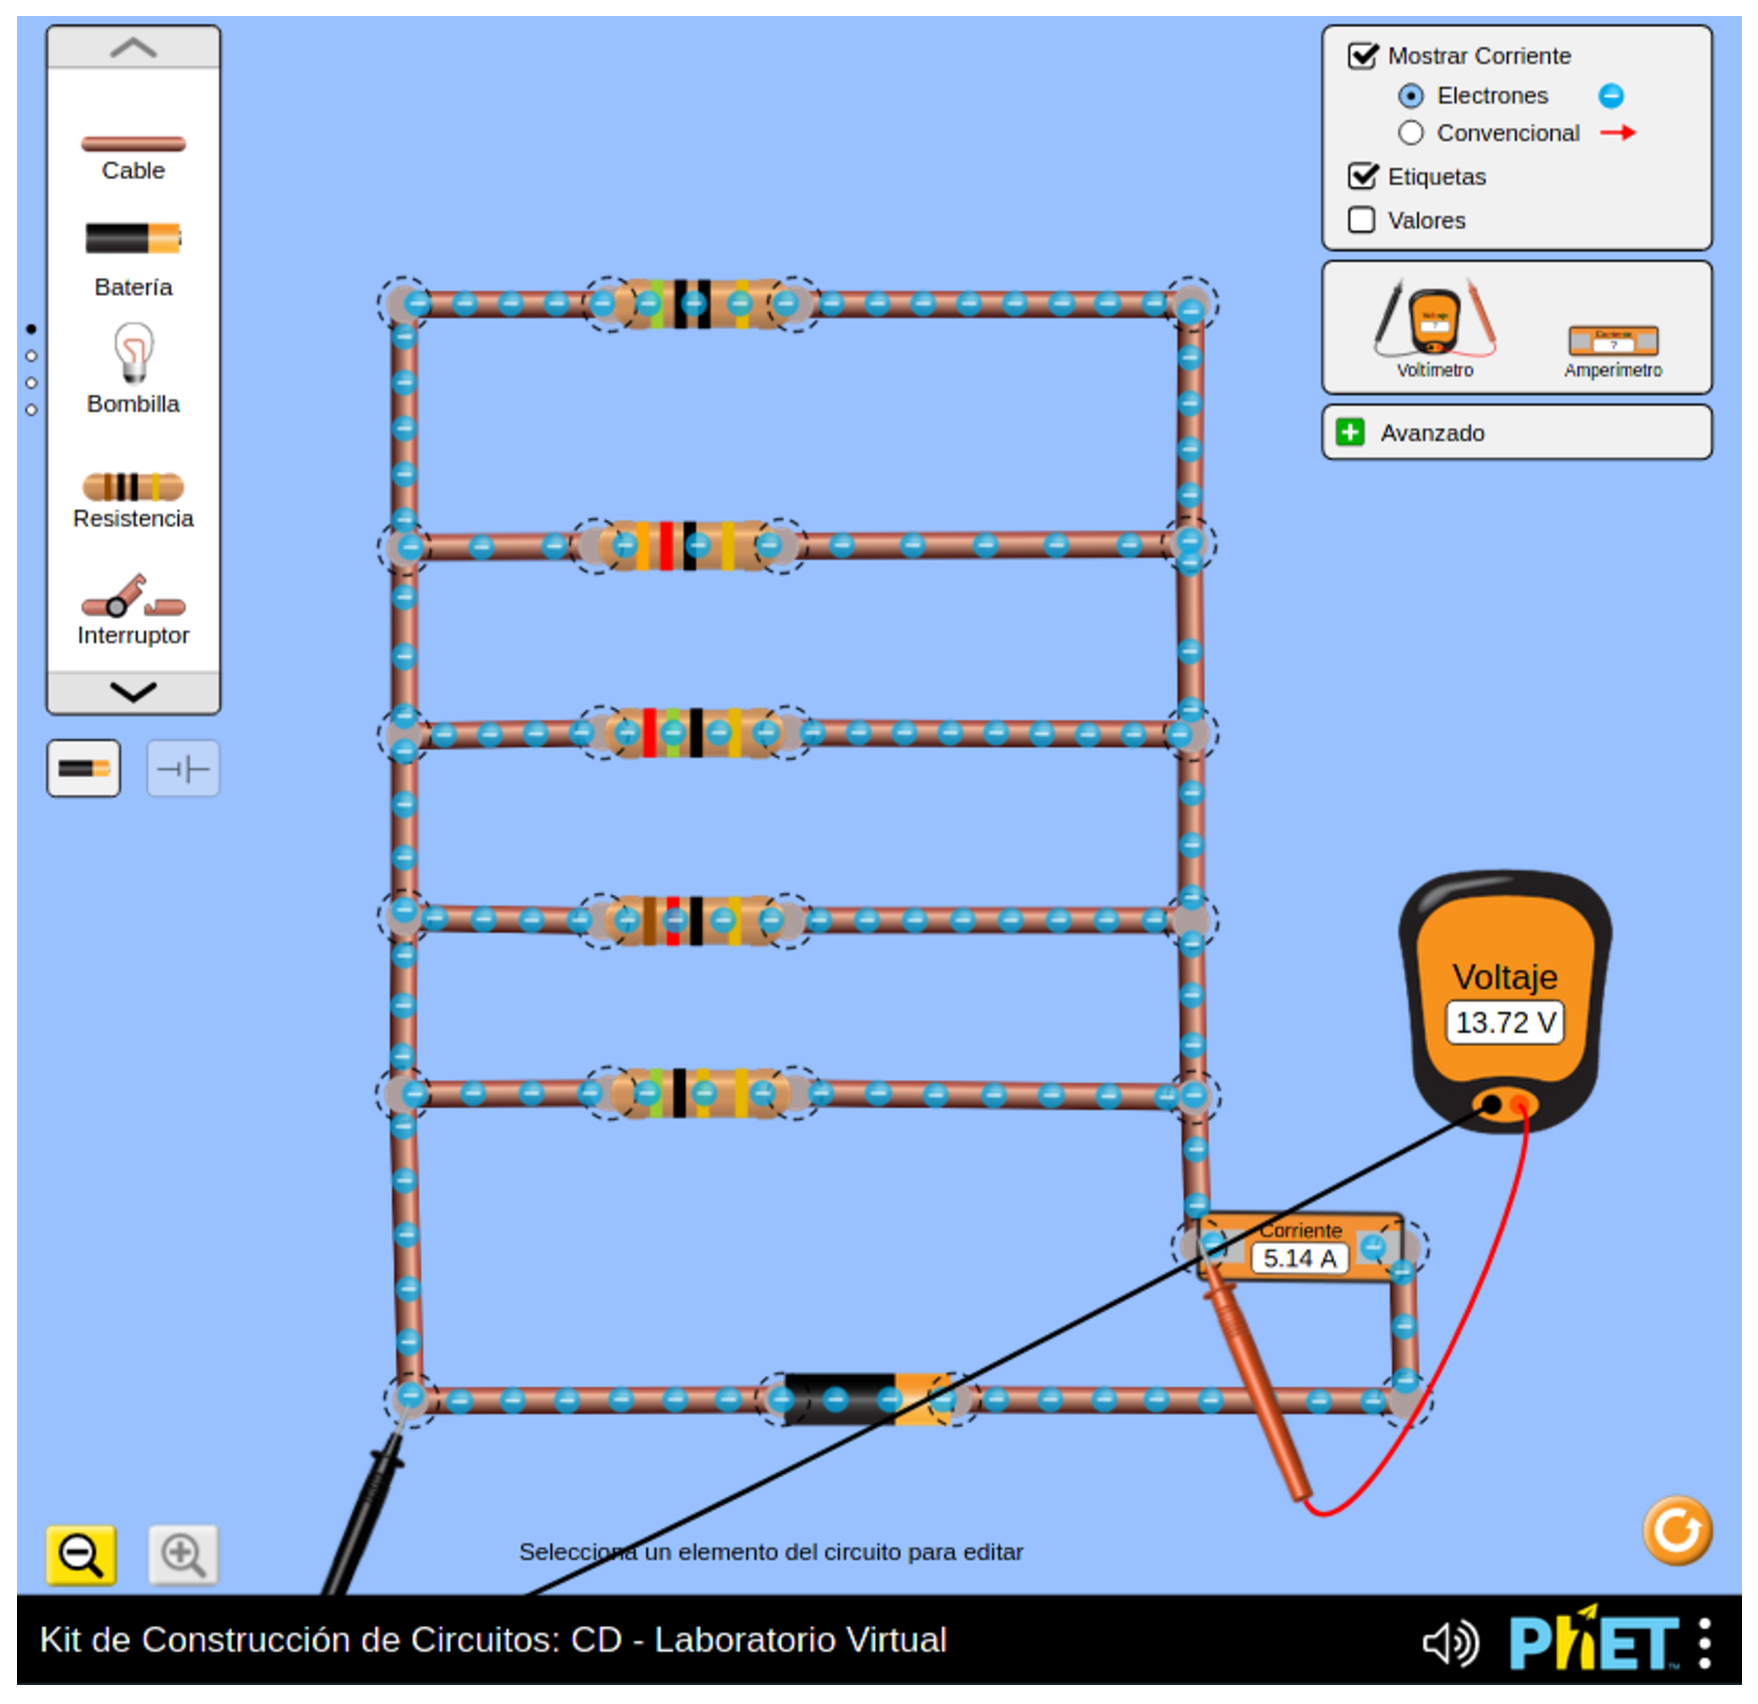
\includegraphics[scale=0.45]{resources/figura4.eps}
\caption{Armado de resistencias en paralelo.}
\label{figura4}
\end{figure}

\section{Resultados}

\subsection{Voltímetro - amperímetro}

\begin{center}
\begin{tabular}{|c|>{\centering}m{1.5cm}<{\centering}
                  |>{\centering}m{2.2cm}<{\centering}
                  |>{\centering}m{2.2cm}<{\centering}|}
\hline
& $V [V]$ & $I [A]$ & $R [\Omega]$ \tabularnewline \hline
$R_a$ & 23.08 & 0.46 & 50.17 \tabularnewline \hline
$R_b$ & 22.59 & 0.71 & 31.82 \tabularnewline \hline
$R_c$ & 22.22 & 0.89 & 24.97 \tabularnewline \hline
$R_d$ & 20.57 & 1.71 & 12.03 \tabularnewline \hline
$R_e$ & 17.14 & 3.43 &  5.00 \tabularnewline \hline
\end{tabular}
\end{center}

\subsection{Código de colores}

\begin{center}
\begin{tabular}{|c|>{\centering}m{2.2cm}<{\centering}
                  |>{\centering}m{2.2cm}<{\centering}
                  |>{\centering}m{2.2cm}<{\centering}
                  |>{\centering}m{2.6cm}<{\centering}
                  |>{\centering}m{2.2cm}<{\centering}|}
\hline
& a & b & c & d & $R [\Omega]$ \tabularnewline \hline
$R_a$ & Verde($5$)    & Negro($0$)  & Negro ($0$) & Dorado ($\pm 5\%$) & $(50 \pm 2.5)$  \tabularnewline \hline
$R_b$ & Naranja ($3$) & Rojo ($2$)  & Negro ($0$) & Dorado ($\pm 5\%$) & $(32 \pm 1.6)$  \tabularnewline \hline
$R_c$ & Rojo ($2$)    & Verde ($5$) & Negro ($0$) & Dorado ($\pm 5\%$) & $(25 \pm 1.25)$ \tabularnewline \hline
$R_d$ & Marrón ($1$)  & Rojo ($2$)  & Negro ($0$) & Dorado ($\pm 5\%$) & $(12 \pm 0.6)$  \tabularnewline \hline
$R_e$ & Verde ($5$)   & Negro ($0$) & Oro ($0.1$) & Dorado ($\pm 5\%$) & $( 5 \pm 0.25)$ \tabularnewline \hline
\end{tabular}
\end{center}

\subsection{Puente de \emph{Wheatstone}}

\begin{center}
\begin{tabular}{|c|>{\centering}m{1.5cm}<{\centering}
                  |>{\centering}m{2.2cm}<{\centering}
                  |>{\centering}m{2.2cm}<{\centering}
                  |>{\centering}m{2.2cm}<{\centering}|}
\hline
& $R_2 [\Omega]$ & $R_3 [\Omega]$ & $R_4 [\Omega]$ & $R_x [\Omega]$ \tabularnewline \hline
$R_a$ & 21.4 & 70.0 &  30.0 & 49.93 \tabularnewline \hline
$R_b$ & 75.0 & 40.0 &  93.7 & 32.02 \tabularnewline \hline
$R_c$ & 68.0 & 19.5 &  53.0 & 25.02 \tabularnewline \hline
$R_d$ & 31.5 & 29.0 &  76.0 & 12.02 \tabularnewline \hline
$R_e$ & 42.9 & 14.0 & 120.0 &  5.00 \tabularnewline \hline
\end{tabular}
\end{center}

\subsection{Resumen general}
Valores obtenidos por los diferentes métodos:

\begin{center}
\begin{tabular}{|c|>{\centering}m{3.5cm}<{\centering}
                  |>{\centering}m{3.5cm}<{\centering}
                  |>{\centering}m{3.5cm}<{\centering}|}
\hline
$R [\Omega]$ & Voltímetro-amperímetro & Código de colores & Puente de \emph{Wheatstone} \tabularnewline \hline
$R_a$ & 50.17 & $(50 \pm 2.5)$  & 49.93 \tabularnewline \hline
$R_b$ & 31.82 & $(32 \pm 1.6)$  & 32.02 \tabularnewline \hline
$R_c$ & 24.97 & $(25 \pm 1.25)$ & 25.02 \tabularnewline \hline
$R_d$ & 12.03 & $(12 \pm 0.6)$  & 12.02 \tabularnewline \hline
$R_e$ &  5.00 & $( 5 \pm 0.25)$ &  5.00 \tabularnewline \hline
\end{tabular}
\end{center}

\subsubsection{Combinación de resistencias}
Los valores teóricos de la resistencia eléctrica de la combinación en serie y en
paralelo son:

\begin{equation*}
    R_{eq} (serie) = 50 + 32 + 25 + 12 + 5 = 124.0 [\Omega]
\end{equation*}
\begin{equation*}
    \frac{1}{R_{eq}} (paralelo) = \frac{1}{50} + \frac{1}{32} + \frac{1}{25} + \frac{1}{12} + \frac{1}{5} = 0.3746
\end{equation*}
\begin{equation*}
    R_{eq} (paralelo) = 2.6696 [\Omega]
\end{equation*}

Los valores experimentales de la resistencia eléctrica de la combinación en
serie y en paralelo son:

\begin{equation*}
    R_{eq} (serie) = \frac{V}{I} = \frac{23.62}{0.19} = 124.32 [\Omega]
\end{equation*}
\begin{equation*}
    R_{eq} (paralelo) = \frac{V}{I} = \frac{13.72}{5.14} = 2.67 [\Omega]
\end{equation*}

\end{document}

